%=========================================
% 	   Einleitung     		 =
%=========================================
\chapter{RN Versuch}
\section{Versuchsaufbau}
Der Aufbau des Versuchs besteht aus zwei Routern, einem Switch, zwei Host Rechnern und den entsprechenden Kabeln. Vor Beginn des Versuchs werden sowohl die Switche, als auch die Router auf ihre Werkseinstellungen zur�ck gesetzt. Damit wird sichergestellt, dass eventuelle Konfigurationen aus vorangegangen Versuchen gel�scht werden und keine Fehler verursachen.

Nachdem die Hardware vorbereitet ist, werden die Adressen aus einem gegebenen Netz errechnet. Gegeben ist das Netz 192.168.1.0/24. Dieses soll in ein Netz mit max. 120 Hosts, ein Netz mit max.  60 Hosts aufgeteilt werden. Das gr��ere Netz soll mit dem Router R1 verbunden werden, das Kleinere soll mit dem Router R2 verbunden werden. Da die Router sich in dieser Konfiguration in verschiedenen Netzen befinden, muss noch ein Transfernetz eingerichtet werden, damit sie untereinander kommunizieren sollen. Aus diesen Anforderungen ergeben sich die drei Netze, die in der Tabelle \ref{tab:berechneteNetzwerke}.

\begin{table}[h]
\begin{tabular}{|*{2}{c|} p{0.15\linewidth}|*{3}{c|}}
\hline
Netzadresse & BC & Hosts & Subnet Mask & Slash & Adressen\\
\hline
\hline
192.168.0.1 & 192.168.1.127 & 192.168.1.1 - 192.168.1.126 & 255.255.255.128 & /25 & 126 \\
\hline
192.168.0.128 & 192.168.1.191 & 192.168.1.129 - 192.168.1.190 & 255.255.255.192 & /26 &62 \\
\hline
192.168.0.192 & 192.168.1.199 & 192.168.1.193 - 192.168.1.198 & 255.255.255.248 & /29 &6	 \\
\hline
\end{tabular}
\caption{Die berechneten Netzwerke}
\label{tab:berechneteNetzwerke}
\end{table}

Nach dieser Berechnung kann eine �bersicht aufgestellt werden, wie das Netzwerk aufgebaut werden soll. Die Adressvergabe ist in Tabelle \ref{tab:berechneteNetzwerke} dargestellt.
\begin{table}[H]
\begin{tabular}{|*{5}{c|}}
\hline
Device & Host Name & Interface & IP Address & Subnet Mask \\
\hline
R1 & R1 & Serial 0/0/0(DCE) & 192.168.1.193 & 255.255.255.248 \\
\hline
& & FE 0/0 & 192.168.1.1 & 255.255.255.128 \\
\hline
H1 &H1 &  Ethernet & 192.168.1.2 & 255.255.255.128 \\
\hline
H2 & H2 & Ethernet & 192.168.1.130 & 255.255.255.192 \\
\hline
R2 & R2 & Serial 0/0/0(DTE) & 192.168.1.194 &255.255.255.248 \\
\hline
& & FE 0/0 & 192.168.1.129 & 255.255.255.192\\
\hline
\end{tabular}
\caption{Der Aufbau des Netzwerks}
\label{tab:aufbauNetzwerk}
\end{table}


\begin{figure}[H] 
  \centering
     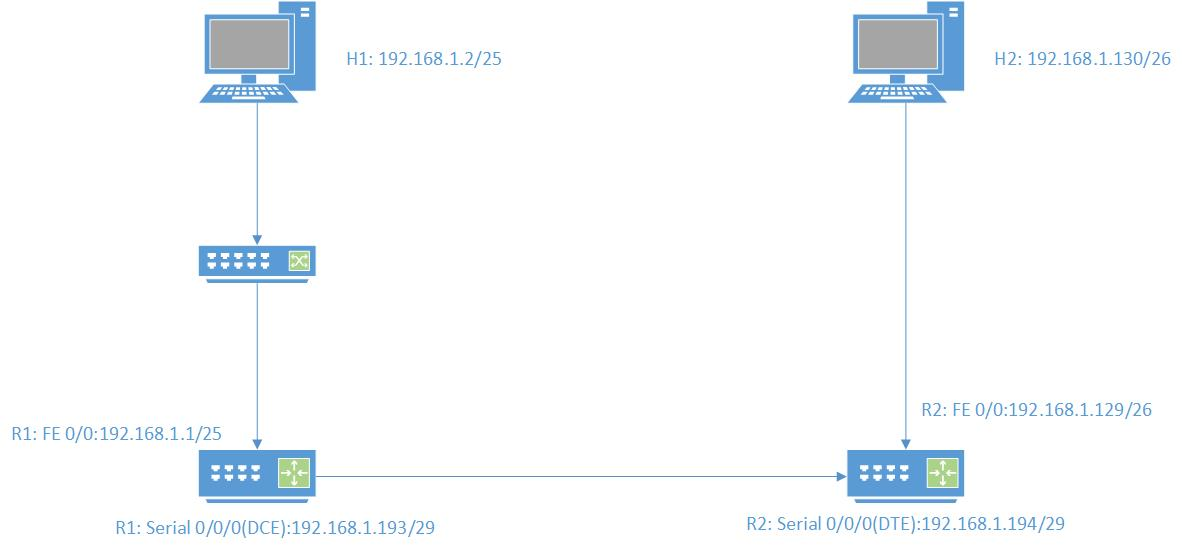
\includegraphics[width=1\textwidth]{tkinhalt/rn_bilder/rn.jpg}
  \caption{Der Aufbau unseres Netzwerks}
  \label{fig:aufbauNW}
\end{figure}

Nachdem die Netze berechnet sind werden sowohl Router als auch Hosts entsprechend eingerichtet.

\section{Routing}
\subsection{�berpr�fung der Routingeinstellungen}
Der Befehl \textit{show ip route} zeigt die Routen an, die der Router gespeichert hat.
\begin{lstlisting}[captionpos=b,caption=Die Routing Table von R1]
R1#show ip route
Codes: C - connected, S - static, R - RIP, M - mobile, B - BGP
       D - EIGRP, EX - EIGRP external, O - OSPF, IA - OSPF inter area 
       N1 - OSPF NSSA external type 1, N2 - OSPF NSSA external type 2
       E1 - OSPF external type 1, E2 - OSPF external type 2
       i - IS-IS, su - IS-IS summary, L1 - IS-IS level-1, L2 - IS-IS level-2
       ia - IS-IS inter area, * - candidate default, U - per-user static route
       o - ODR, P - periodic downloaded static route

Gateway of last resort is not set

     192.168.1.0/24 is variably subnetted, 2 subnets, 2 masks
C       192.168.1.0/25 is directly connected, FastEthernet0/0
C       192.168.1.192/29 is directly connected, Serial0/0/0
\end{lstlisting}

\begin{lstlisting}[captionpos=b,caption=Die Routing Table von R2]
R2#show ip route
Codes: L - local, C - connected, S - static, R - RIP, M - mobile, B - BGP
       D - EIGRP, EX - EIGRP external, O - OSPF, IA - OSPF inter area
       N1 - OSPF NSSA external type 1, N2 - OSPF NSSA external type 2
       E1 - OSPF external type 1, E2 - OSPF external type 2
       i - IS-IS, su - IS-IS summary, L1 - IS-IS level-1, L2 - IS-IS level-2
       ia - IS-IS inter area, * - candidate default, U - per-user static route
       o - ODR, P - periodic downloaded static route, + - replicated route

Gateway of last resort is not set

      192.168.1.0/24 is variably subnetted, 4 subnets, 3 masks
C        192.168.1.128/26 is directly connected, FastEthernet0/0
L        192.168.1.129/32 is directly connected, FastEthernet0/0
C        192.168.1.192/29 is directly connected, Serial0/0/0
L        192.168.1.194/32 is directly connected, Serial0/0/0
\end{lstlisting}

Der Router hat keine Route in das Netzwerk 192.168.1.128. Dieses Netzwerk kann er nicht direkt erreichen und eingestellt ist auch keine.

Ob die beiden Router eine Verbindung zueinander haben kann mit einem Ping getestet werden:
\begin{lstlisting}[captionpos=b,caption=Ping von R1 zu R2]
R1#ping 192.168.1.129

Type escape sequence to abort.
Sending 5, 100-byte ICMP Echos to 192.168.1.129, timeout is 2 seconds:
.....
Success rate is 0 percent (0/5)
\end{lstlisting}


Dieser Ping war nicht erfolgreich.

Ein Ping wird auch von H1 zu H2 ausgef�hrt. Dieser Ping ist auch nicht erfolgreich.

Dass beide Pings nicht erfolgreich waren liegt daran, dass sich die die Router, bzw. die Pc je in unterschiedlichen Netzwerken befunden haben. Da noch keine Routen konfiguriert waren, konnten die Router die Datenpakete nicht weiterleiten.

\subsection{Einstellen des Routingprotokolls}
RIP ist ein Interieur Gateway Protokoll, also ein Routing Protokoll, das innerhalb eines autonomen Netzes benutzt wird. Dieses Protokoll ist in der Lage eine eigene Routingtabelle aufzubauen. Dadurch bleibt das Netzwerk flexibel und muss beim Einbau von neuen Ger�ten nicht neu konfiguriert werden. Da wird in unserem Netzwerk verschiedene und klassenlose Netzmasken nutzen m�ssen wir RIP v2 nutzen.
Der Befehl \textit{router rip} aktiviert das RIP routing und versetzt den Router in den Konfigurationsmodus. Mit dem Befehl \textit{version 2} konfiguriert man die Software dass sie nur noch RIP v2 Pakete empf�ngt und aussendet. Der Befehl \textit{network 192.168.1.0} wei�t dem Netzwerk 192.168.1.0 das Routing Protokoll zu. Der Router 1 wird mit der Befehlssequenz
\begin{lstlisting}[captionpos=b,caption=Befehlssequenz zum Konfigurieren von R1]
R1(config)#router rip 
R1(config-router)# version 2 
R1(config-router)# network 192.168.1.0
R1# copy running-config startup-config
\end{lstlisting} zum Routen eingerichtet. Die letzte Zeile speichert die neuen Einstellungen in den NVRAM.

R2 wird analog konfiguriert.

\subsection{�berpr�fen der Routing Einstellungen}
Nach dem Einstellen der Routing Konfiguration kann diese wieder �berpr�ft werden. 

\begin{lstlisting}[captionpos=b,caption=Die Ausgabe der Routingseinstellungen von R1]
R1#show ip route 
Codes: C - connected, S - static, R - RIP, M - mobile, B - BGP
       D - EIGRP, EX - EIGRP external, O - OSPF, IA - OSPF inter area 
       N1 - OSPF NSSA external type 1, N2 - OSPF NSSA external type 2
       E1 - OSPF external type 1, E2 - OSPF external type 2
       i - IS-IS, su - IS-IS summary, L1 - IS-IS level-1, L2 - IS-IS level-2
       ia - IS-IS inter area, * - candidate default, U - per-user static route
       o - ODR, P - periodic downloaded static route

Gateway of last resort is not set

     192.168.1.0/24 is variably subnetted, 3 subnets, 3 masks
C       192.168.1.0/25 is directly connected, FastEthernet0/0
C       192.168.1.192/29 is directly connected, Serial0/0/0
R       192.168.1.128/26 [120/1] via 192.168.1.194, 00:00:20, Serial0/0/0
\end{lstlisting}

In der Routingtabelle werden die Netzwerke 192.168.1.0/25 , 192.168.1.192/29 und 192.168.1.128/26 angezeigt. Das \glqq R\grqq~bedeutet, dass dieses Netzwerk �ber RIP, also durch Routing erreicht werden kann. \glqq via 192.168.1.194\grqq~bedeutet, dass diese Adresse  �ber die Adresse 192.168.1.194 erreicht werden kann. Diese Adresse ist dann das Gateway um in das Netz 192.168.1.128 zu erreichen. Serial 0/0/0 gibt an, �ber welchen Port des Routers das Netzwerk erreicht werden kann.


\begin{lstlisting}[captionpos=b,caption=Die Ausgabe der Routingseinstellungen von R2]
R2#show ip route
...

      192.168.1.0/24 is variably subnetted, 5 subnets, 4 masks
R        192.168.1.0/25 [120/1] via 192.168.1.193, 00:01:14, Serial0/0/0
C        192.168.1.128/26 is directly connected, FastEthernet0/0
L        192.168.1.129/32 is directly connected, FastEthernet0/0
C        192.168.1.192/29 is directly connected, Serial0/0/0
L        192.168.1.194/32 is directly connected, Serial0/0/0
\end{lstlisting}

In der Routingtabelle von R2 sind die Netzwerke 192.168.1.0, 192.168.1.128 und 192.168.1.192 aufgef�hrt. 

Ob die Routingeinstellungen tats�chlich funktionieren, kann wieder mit Pings getestet werden. Dieses Mal sind die Pings erfolgreich. Der Grund ist, dass die Router nun ein Routingprotokoll konfiguriert und Informationen haben, wie sie das jeweils andere Interface erreichen. 

\subsection{�berpr�fung der RIP Kommunikation}
\begin{lstlisting}
*Jun 18 12:27:33.923: RIP: build update entries
*Jun 18 12:27:33.923:   192.168.1.128/26 via 0.0.0.0, metric 2, tag 0
*Jun 18 12:27:33.923:   192.168.1.192/29 via 0.0.0.0, metric 1, tag 0
\end{lstlisting}
Der Befehl \textit{debug ip rip} aktiviert die Ausgabe der Rip Kommunikation eines Routers. Mit diesem Befehl kann mitgelesen werden, welche Informationen zwischen den Routern ausgeteilt werden. Auff�llig ist, dass alle RIP Informationen �ber das Interface 0.0.0.0 geschickt werden. Diese Adresse bezeichnet das Defaultgateway, bzw. alle Netze, die unbekannt sind werden mit dieser Adresse belegt.

Was noch auff�llt ist, dass die Netze unterschiedliche Metriken haben. Die unterschiedlichen Metriken ergeben sich aus der Route, die gew�hlt werden muss. Das Netzwerk 192.168.1.192/29 kann direkt vom Router R1 erreicht werden. Um das Netzwerk 192.168.1.128/26  zu erreichen muss der Router den Umweg �ber das Netzwerk 192.168.1.192 nehmen. Die Metrik von Rip v2 sagt aus, wie viele Hops eine Route hat.
Da wir uns beim einteilen des Netzwerkes zwischen den 2 Routern vertan haben, statt /30 haben wir /29 benutzt, kann es zu Abweichungen zur Aufgabenstellung kommen. Erinnern wir uns an die Grafik \ref{fig:aufbauNW} wird schnell klar, warum die Routen unterschiedliche Metriken haben.

\subsection{Reflection}
a. What would happen to the routing table on router R1 if the Ethernet network on router R2 went down? Configure this case and analyze.
\todo{a}


b. What would happen if router R1 was configured to run RIPv1, and R2 was configured to run RIPv2? Configure this case and analyze with show ip route and debug ip rip.

R1 would ignore all sent RIP v2 information and send out RIP v1 information.
\begin{lstlisting}
*Jun 18 12:33:51.091: RIP: ignored v2 packet from 192.168.1.194 (illegal version)
*Jun 18 12:33:55.343: RIP: sending v1 update to 255.255.255.255 via FastEthernet0/0 (192.168.1.1)
\end{lstlisting}
